
\section{Messung} % (fold)
\label{sec:messung}
\FloatBarrier
Im Folgenden wird zunächst die Stärke des Magnetfeldes bestimmt. 
Anschließend wird die Faraday-Rotation bestimmt und daraus die Masse der freien Elektronen.

Aufgrund der starken Schwankungen der Messpunkte wird auf eine Fehlerrechnung verzichtet.

\subsection{Bestimmung der Magnetfeldstärke} % (fold)
\label{sub:bestimmung_der_magnetfeldstärke}

Die zur Bestimmung der Magnetfeldstärke verwendeten Daten sind in Tabelle \ref{tab_mag} dargestellt.
Zur Bestimmung des Mittelpunktes der symmetrischen Kurve wurde sowohl eine Ausgleichrechung mithilfe einer Gauß-, als auch einer Lorentz-Funktion durchgeführt (Abbildung \ref{fig_mag}).
Beide Funktionen haben ihren Mittelpunkt bei
\begin{equation*}
	z_\text{max} \approx \SI{29.74}{\milli\meter}.
\end{equation*}

Somit bestimmt sich die Magnetfeldstärke zu
\begin{equation*}
	B(z_\text{max}) \approx \SI{455}{\milli\tesla},
\end{equation*}
welche im weiteren Verlauf der Rechnung verwendet wird.

\begin{figure}
	\centering
	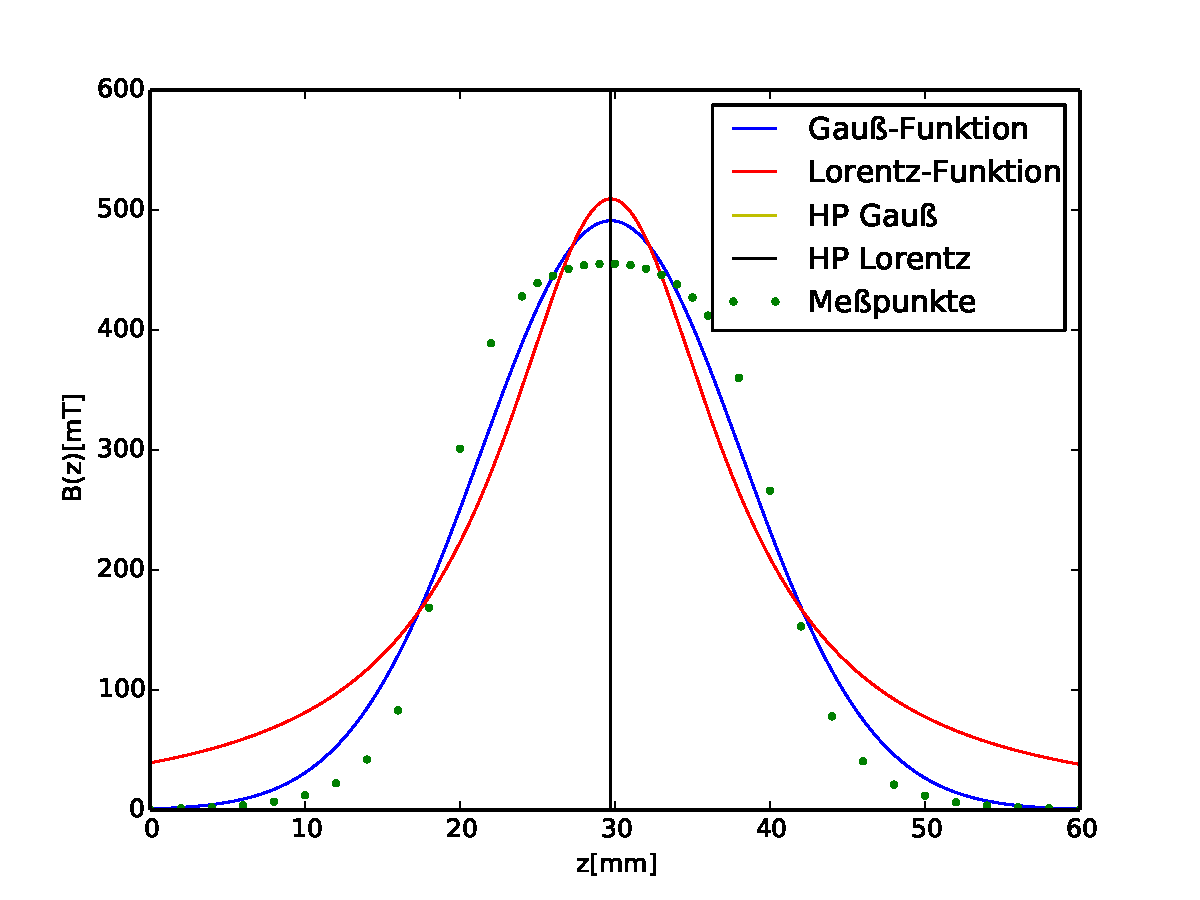
\includegraphics[width = 14cm]{data/gauss.pdf}
	\caption{Messpunkte und Ausgleichsrechnungen zur Bestimmung der Magnetfeldstärke.}
	\label{fig_mag}
\end{figure}

\begin{table}
	\centering
	\caption[]{Zur Bestimmung der Magnetfeldstärke verwendete Messpunkte.}
	\begin{tabular}{r r r r}
		\toprule
		d[$\SI{}{\milli\meter}$] & B[$\SI{}{\milli\tesla}$] & d[$\SI{}{\milli\meter}$] & B[$\SI{}{\milli\tesla}$]\\
		\midrule
		 0	&	  0.80	&	30	&	455.00\\
		 2	&	  1.28	&	31	&	454.00\\
		 4	&	  2.19	&	32	&	451.00\\
		 6	&	  3.81	&	33	&	446.00\\
		 8	&	  6.86	&	35	&	427.00\\
		10	&	 12.24	&	36	&	412.00\\
		12	&	 22.40	&	38	&	360.00\\
		14	&	 42.10	&	40	&	266.00\\
		16	&	 83.00	&	42	&	153.00\\
		18	&	168.60	&	44	&	 78.00\\
		20	&	301.00	&	46	&	 40.60\\
		22	&	389.00	&	48	&	 21.20\\
		24	&	428.00	&	50	&	 11.90\\
		25	&	439.00	&	52	&	  6.60\\
		26	&	445.00	&	54	&	  3.76\\
		27	&	451.00	&	56	&	  2.19\\
		28	&	454.00	&	58	&	  1.31\\
		29	&	455.00	&	60	&	  0.82\\
		\bottomrule
	\end{tabular}
	\label{tab_mag}
\end{table}
\FloatBarrier
\subsection{Bestimmung der Masse von freien Elektronen} % (fold)
\label{sub:bestimmung_der_masse_von_freien_elektronen}

Die zur berechnung der Masse freier Elektronen verwendeten Daten sind in Tabelle \ref{tab_1} bis \ref{tab_2} dargestellt.
Zunächst werden die Winkel in rad umgerechnet wobei
\begin{eqnarray*}
	1\SI{}{\arcsecond} &=& \frac{\pi}{648000}\SI{}{\radian},\\
	1\SI{}{\degree} &=& \frac{\pi}{180}\SI{}{\radian}
\end{eqnarray*}
gilt.

Anschließend wird der Winkel noch auf die Dicke $D$ der Probe normiert und die Winkel der hochreinen Probe von den Winkeln der anderen beiden Proben abgezogen.
Somit ergeben sich die Winkel aus Tabelle \ref{wink1}

Mit dieser Methode sollte nur der Anteil der n-dotierung übrig bleiben, welcher aus den zu untersuchenden freien Elektronen besteht.
Die Daten der Proben sind in Tabelle \ref{data} aufgeführt.

Aus dem Winkel lässt sich mithilfe einer linearen Regression mit
\begin{equation*}
	\frac{\Theta}{D} = m_\text{reg} \lambda^2 + b
\end{equation*}
die Masse der Elektronen über Gleichung \eqref{eqn:theta_final} bestimmt werden.
In dieser Gleichung ist der frequenzabhängige Brechungsindex $n$ vorhanden. Da die frequenzabhängigkeit nicht berücksichtigt werden soll und sich die Werte von etwa $3.3-3.5$ (\cite{GeAs}) erstrecken wird ein Brechungsindex von 
\begin{equation*}
	n = 3.4
\end{equation*}
angenommen.
Die Regression lieferte 
\begin{eqnarray*}
	m_\text{dünn} &=& \SI{2.17e13}{1\per\meter^3},\\
	m_\text{dick} &=& \SI{-1.81e11}{1\per\meter^3}
\end{eqnarray*}
und ist in Abbildung \ref{fit} dargestellt.

Daraus ergiebt sich für die Masse der freien Elektronen
\begin{eqnarray*}
	m_{\text{elek}_\text{dünn}} &=& \SI{6.14e-32}{\kilogram},\\
	m_{\text{elek}_\text{dick}} &=& \SI{4.40e-31}{\kilogram}.
\end{eqnarray*}
Der Quotient aus errechneten Masse eines freien Elektrons und der Masse eines gebundenen ELektrons ($m_e = \SI{9.11e-31}{\kilogram}$) sollte nach Litartur $m/m_e \approx 0.066$ ergeben \cite{kittel}.
In diesem Fall erreicht der Quotient die Werte
\begin{eqnarray*}
	\frac{m_{\text{elek}_\text{dünn}}}{m_\text{e}} &=& \SI{0.0675}{},\\
	\frac{m_{\text{elek}_\text{dick}}}{m_\text{e}} &=& \SI{0.4833}{}.
\end{eqnarray*}
und weicht der Wert für die Masse der Elektronen bei der dünnen Probe um etwa $\SI{2.16}{\percent}$ und die Masse der Elektronen bei der dicken Probe $\SI{86.35}{\percent}$ ab.

\begin{table}
	\centering
	\caption{Daten der verwendeten Proben.}
	\begin{tabular}{r r r}
	\toprule
		Probe & D[$\SI{}{\milli\meter}$]& N[$\SI{e18}{1\per\centi\meter^3}$]\\ 
		\midrule
		GeAs hochrein & 5.11 & 0\\
		GeAs n-dotiert dünn & 1.296 & 2.8\\
		GeAs n-dotiert dick & 1.460 & 1.2\\
	\end{tabular}
\end{table}

\begin{figure}
\centering
	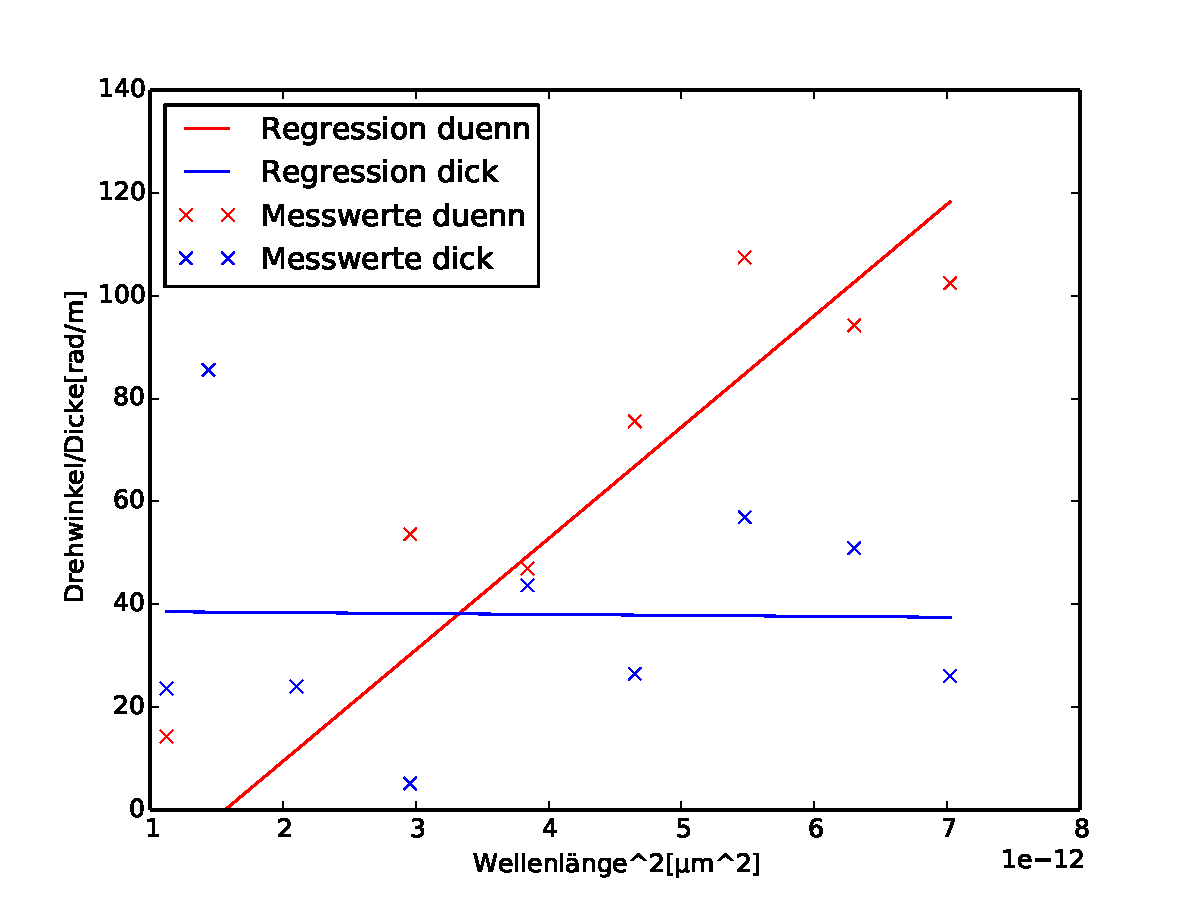
\includegraphics[width = 14cm]{data/fit.pdf}
	\caption{Lineare Ausgleichsrechnung.}
	\label{fit}
\end{figure}

\begin{table}
	\centering
	\caption{Drehwinkel der n-dotierten Proben, nachdem der Winkel der hochreinen Probe abgezogen wurde.}
	\begin{tabular}{r r}
		GeAs n-dotiert dünn & GeAs n-dotiert dick\\
		\hline 
		$\Theta_\text{dünn}[\SI{}{\radian\per\meter}]$ & $\Theta_\text{dick}[\SI{}{\radian\per\meter}]$\\
		\hline\hline
		102.42	&	 26.04\\
		 94.23	&	 50.89\\
		107.44	&	 56.92\\
		 75.55	&	 26.51\\
		 46.94	&	 43.68\\
		 53.59	&	  5.16\\
		 -7.11	&	 24.01\\
		-35.89	&	 85.58\\
		 14.30	&	 23.62\\
		 \hline
	\end{tabular}
	\label{wink1}
\end{table}

\begin{table}
	\centering
	\caption[]{Drehwinkel der hochreinen Probe.}
	\begin{tabular}{r c r r }
		Filter[$\SI{}{\micro\meter}$] & Polarisation & Winkel[$\SI{}{\degree}$] & Winkel[$\SI{}{\arcsecond}$]\\
		\hline\hline
		2.650	&	+	&	194	&	51\\
				&	-	&	205	&	55\\
		2.510	&	+	&	197	&	33\\
				&	-	&	201	&	59\\
		2.340	&	+	&	194	&	 3\\
				&	-	&	202	&	 2\\
		2.156	&	+	&	194	&	52\\
				&	-	&	201	&	42\\
		1.960	&	+	&	192	&	40\\
				&	-	&	204	&	15\\
		1.720	&	+	&	192	&	58\\
				&	-	&	204	&	31\\
		1.450	&	+	&	191	&	 4\\
				&	-	&	207	&	42\\
		1.200	&	+	&	184	&	36\\
				&	-	&	209	&	35\\
		1.060	&	+	&	179	&	 5\\
				&	-	&	214	&	55\\
		\hline
	\end{tabular}
	\label{tab_1}
\end{table}

\begin{table}
	\centering
	\caption[]{Drehwinkel der dünnen Probe.}
	\begin{tabular}{r c r r }
		Filter[$\SI{}{\micro\meter}$] & Polarisation & Winkel[$\SI{}{\degree}$] & Winkel[$\SI{}{\arcsecond}$]\\
		\hline\hline
		2.650	&	+	&	187	&	 2\\
				&	-	&	205	&	 3\\
		2.510	&	+	&	192	&	 1\\
				&	-	&	207	&	39\\
		2.340	&	+	&	191	&	57\\
				&	-	&	209	&	 0\\
		2.156	&	+	&	192	&	20\\
				&	-	&	205	&	 3\\
		1.960	&	+	&	193	&	 0\\
				&	-	&	203	&	44\\
		1.720	&	+	&	194	&	 7\\
				&	-	&	205	&	10\\
		1.450	&	+	&	194	&	13\\
				&	-	&	197	&	30\\
		1.200	&	+	&	195	&	50\\
				&	-	&	194	&	11\\
		1.060	&	+	&	192	&	38\\
				&	-	&	203	&	54\\
		\hline
	\end{tabular}
	\label{tab_2}
\end{table}

\begin{table}
	\centering
	\caption[]{Drehwinkel der dicken Probe.}
	\begin{tabular}{r c r r }
		Filter[$\SI{}{\micro\meter}$] & Polarisation & Winkel[$\SI{}{\degree}$] & Winkel[$\SI{}{\arcsecond}$]\\
		\hline\hline
		2.650	&	+	&	194	&	59\\
				&	-	&	201	&	 7\\
		2.510	&	+	&	193	&	40\\
				&	-	&	202	&	32\\
		2.340	&	+	&	195	&	49\\
				&	-	&	206	&	46\\
		2.156	&	+	&	195	&	27\\
				&	-	&	201	&	 6\\
		1.960	&	+	&	193	&	 4\\
				&	-	&	203	&	 2\\
		1.720	&	+	&	196	&	54\\
				&	-	&	200	&	38\\
		1.450	&	+	&	195	&	14\\
				&	-	&	203	&	25\\
		1.200	&	+	&	184	&	46\\
				&	-	&	204	&	15\\
		1.060	&	+	&	191	&	32\\
				&	-	&	204	&	31\\
		\hline
	\end{tabular}
	\label{tab_2}
\end{table}

\section{Diskussion} % (fold)
\label{sec:diskussion}

Alles in allem lässt sich sagen, dass die Apparatur dafür geeignet ist die Masse von freien Elektronen zu bestimmen.
Es ist allerdings anzumerken, dass die Werte für die lineare Ausgleichsrechnung keine linearität vermuten lassen weshalb auch die Fehler nicht berücksichtigt worden sind.
Es ist jedoch gelungen, die Masse der freie Elektronen relativ genau zu bestimmen.
Bei der $\SI{1.296}{\milli\meter}$ dicken Probe konnte so ein Fehler auf die Masse von $\SI{2.16}{\percent}$ erreicht werden, während bei der $\SI{1.36}{\milli\meter}$ dicken Probe der Fehler bei $\SI{86.35}{\percent}$ liegt.
Dominante Fehlerquellen sind die Vernachlässigung der Dispersion des Brechungsindices und dass die Apparatur nicht optimal jusitert werden konnte.